\documentclass[11pt, oneside]{article}   	% use "amsart" instead of "article" for AMSLaTeX format
\usepackage{geometry}
\usepackage[]{algorithm2e}
\geometry{letterpaper}
\usepackage{graphicx}
\usepackage{amssymb}
\usepackage{amsthm}
\usepackage{parskip}
\usepackage{enumitem}
\usepackage{amsmath}
\usepackage{comment}
\usepackage{graphicx}

\graphicspath{ {./images/} }


\title{AlgoProject}
\author{Tianbo Yang, Yitian Cao, Xinran Liu}
%\date{}	

\begin{document}

\maketitle

\section{Abstract}
This paper will present a greedy algorithm to solve the problem of scheduling classes with constraints of room capacity, time conflict, and teacher conflict. This is a NP-hard problem, but our algorithm can achieve polynomial time complexity and approximate the optimal solution. Using random generated and realistic data, our algorithm can achieve 98\% fit percentage of students' preference on average. With real Bryn Mawr registration data in the past, our algorithm can achieve 96.6\% fit percentage on average. All the output schedules are valid. During our experimental analysis, we noticed that room capacity is hardly a significant restriction comparing to time conflict between classes when the student body is under 30000. So we recommend registrar consider the high-conflict classes first and try to schedule them in different time slots.   

\section{Description}
We first calculate the popularity of each class by counting how many students want to take the class. Then we create a 2D conflict matrix called $classConflicts$ with row $c_1,c_2,...c_i$ and column $c_1,c_2,...c_j$ as all the classes. We calculate the conflict number by recording number of students that want to take both $c_i$ and $c_j$ at $classConflicts[i][j]$. If two classes are taught by the same professor, we set the conflict number to $\infty$ Then for each unique $(i,j)$ pair, we create a list that stores all the $(i,j)$ pair in the order of decreasing conflict number. For each pair in the list, we consider both classes in order. If the class is not yet scheduled, at each time slot, we consider 1) number of surplus students at the largest available room; and 2) the sum of conflicts with previous class(es) that are scheduled at this time slot. Schedule the class at $t_k$, where it satisfies the most students who want to take this class and at $c_l$, where it's the smallest room that can take all the prospective students or otherwise the largest available room. 

Once all the classes have been scheduled, we put students into classes according to their preference list as long as those classes don't have conflicts. 

\section{Pseudo Code}
\begin{algorithm}[H]
\SetKwFunction{Scheduling}{Scheduling}
\SetKwProg{Fn}{Function}{}{}
\Fn{\Scheduling{S,C,R,T,P}}{
    %calculate popularity of classes and conflict matrix%
    Initialize a 2D array $classConflicts[c][c]$ where the value of each cell is the conflict number of $class_{row-number}$ and $class_{column-number}$\\
    \For{each student $s_a$}{
        \For{each $c_b \in s_a$'s preference list}{
            c_b.popularity++\\
        }
        \For{each two classes i and j \in $s_a$'s preference list}{
                classConflicts[i][j]++\\
                classConflicts[j][i]++\\
        }
    }
    \For{each professor}{
        a = prof[i].firstClass\\
        b = prof[i].secondClass\\
        classConflicts[a][b]++\\
        classConflicts[b][a]++\\
    }
    Create a list $conflict$ that store all the unique class pairs\\
    Sort the list in the order of decreasing conflict number\\
    Sort the rooms by their capacity\\
    \For{each class pair in the conflict list}{
        \For{each class $c_k$ of the two classes}{
            \If{$c_k$ is not scheduled}{
                \For{i = 1 to t}{
                    largeRoom = the largest available room at t_i\\
                    %?%
                    surplus = c_k.popularity - largeRoom.capacity\\
                    sumOfConflict = $\sum$ conflicts of all previous scheduled classes\\
                    finalConflict[i] = max(surplus, sumOfConflict)\\
                }
                Schedule $c_k$ at $t_i$ where we have minimum finalConflict[i]\\
                Schedule $c_k$ at the smallest room at $t_i$ that can either fit all students want to take $c_k$, or the largest available room at $t_i$\\
            }
        }
    }
    
    \For{each student $s_a$}{
        \For{each $c_b \in s_a$'s preference list}{
            \If{$c_b$ is not filled and $s_a$ is available at $c_b$'s class time}{
                register $s_a$ into $c_b$\\
            }
        }
    }
}

\end{algorithm}

\section{Time Analysis}
Creating the 2D array $classConflicts$ requires $O(1)$, because the java array is filled out by default.

The first $for$ loop will loop through all the students, and check each student's 4 preference classes and each unique class pairs, which requires $4s + 6s = 10s$ iterations. Because there is only 4 classes in a student's preference list and the total number of unique class pairs in a student's preference list is ${4 \choose 2} = 6$. Everything inside the loop will be shown that only takes $O(1)$.

We have $\frac{(1+(c-1))\cdot(c-1)}{2} = \frac{c^2-c}{2}$ unique pairs in total, so creating the list of conflicts requires $O(c^2)$. Quick sort is then used to sort the list, which requires $O(c^2 logc^2)$. Sorting the classrooms by their capacity using quick sort again takes $O(rlogr)$. To loop through each unique pair of classes and schedule all the classes requires $c$ iterations. The number of time slots in reality is way fewer than the number of classes, so here we will assume it is a small constant. The $for$ loop that iterates through each time slot requires $t$ loops, but the operation inside will be shown to be $O(r)$. Because classes has to put into $r$ rooms and $t$ timeslots, we will simplify $O(rt)$ as $O(c)$. We will show other operations inside the second $for$ loop takes $O(1)$ or $O(c)$ as well. Overall, the second $for$ loop takes $O(c^2)$ to complete. 

The last $for$ loop and the loop inside will once again check each student's preference list, which runs $4s$ times and is bounded by $O(s)$.

The algorithm's overall time complexity will be $O(c^2logc^2 + s)$ if the following operations can be done in $O(1)$ or $O(c)$ or less than $O(c)$:

\begin{enumerate}
    \item access a student's preference list
    \item increment a class's popularity
    \item check if two classes are taught by the same professor
    \item increment two classes' conflict number 
    \item access class pair in the conflict list
    \item check if a class is scheduled or not
    \item find the largest available room at a given time slot
    \item access class's popularity
    \item access room's capacity
    \item calculate $sumOfConflict$
    \item populate $finalConflict$ array
    \item find the minimum value in $finalConflict$ array
    \item schedule a class at a time slot
    \item find the smallest room at a given time slot that can fit all students who want to take a class
    \item schedule a class at a room 
    \item check if a class is filled 
    \item register a student into a class
    \item check if a student is available at certain time slot
\end{enumerate}


\subsection{Data Structure}
The $student$ class will contain a unique ID, their preference list, and a list of their final registered classes. We can store all the students in an array $students$ by their unique ID. This will allow (1), (17) and (18) to be done in $O(1)$.

The $class$ class will contain a unique ID, its popularity, scheduled room and time slot, an array $finalConflict$ of size $t$, the professor who teaches the class, and an initially empty list $registerationList$. We can store all the classes in an array $classes$ by their unique ID. This will allow (2), (3), (6), (8), (13), and (15) to be done in $O(1)$. 

The $room$ class will contain its capacity and its unique ID. We will create an array of $rooms$ and sort it by the capacity of the rooms (sorting is already being considered in the above analysis). The $timeslot$ class will contain an array called $roomSchedules$, where the index is the room's rank in $rooms$ and the value is the class that is scheduled at this time at certain room. We will store all the time slots in an array $timeSlots$. This will allow (9), (16) to be done in $O(1)$ and (7) to be done in at most $O(r)$. To achieve (14), we need to linearly search each room and access its capacity, then compare it with the popularity of the class, which requires $O(r)$.

The 2D array $classConflicts$ will record the number of conflicts for each pair of different class. The value of $classConflicts[i][j]$ represents the number of conflicts between $class_i$ and $class_j$. This will allow (4) and (5) to be done in $O(1)$. For (10), there is at most $r$ conflict classes at a time slot, therefore calculating the sum of all the conflicts takes $O(r)$. Then, populating final Conflict array, (11), requires $O(rt)$ which can be simplified as $O(c)$. Finding the minimum in this array, (12), takes $O(t) = O(1)$.

\section{Proof of Correctness}
\subsection{Proof of Termination}
The pseudocode and time analysis demonstrated that all the loops run a finite number of iterations. We never check the class again once it's scheduled and we never reconsider a student once we tried to put him or her into all 4 preference list classes. 

\subsection{Proof of Valid Schedule}
\begin{enumerate}
    \item no teacher conflict:
    
    For any two classes $a$ and $b$ that are taught by the same professor, we set its number of conflicts in the 2D array $classConflicts$ to positive infinity. Then, when the algorithm creates the conflict list, these $(a,b)$ pairs will be considered first. Thus, once one of the class, say $a$, is scheduled at some time slot $t_a$, $finalConflict[t_a]$ will be the maximum number in the entire array. But the algorithm will always take the minimum $finalConflict[t]$ to schedule $b$, hence avoiding the situation where two classes taught by the same professor are scheduled at the same time slot. 
    
    \item no room conflict (only one class can be scheduled in the room at a given time):
    
    For each class, we check each time slot once and check the available rooms only once until we schedule the class into one room at a given time. Note that for each time slot we have an array $roomSchedules$ to record which room at the time is occupied. When a class is scheduled, we put the class into the $roomSchedules$ to indicate the room is not available anymore. 
    
    \item all schedulable classes are scheduled (no empty rooms/time slots):
    
    Suppose there is a class $c_d$ that is schedulable, but has not been assigned to a room or time slot. By the algorithm, it must be that all the time slots and rooms is already scheduled, which contradicts the supposition that the class is still schedulable. 
    
    \item no classes are scheduled more than once:
    
    The class pair in the list is unique, and we only look at each unique pair once during the second $for$ loop. Then we only look at classes that are not scheduled, which means scheduled classes will never be looked at again, making sure no classes are scheduled more than once.
    
    \item no enrolled student has a schedule conflict:
    
    Suppose there is a student $s_e$ who has a schedule conflict for two classes $c_a$ and $c_b$ that $s_e$ registered in. Also suppose $s_e$ registered in $c_a$ first. According to the algorithm, it must be that $c_b$ is not filled out and $s_e$ is available at $c_b$'s class time. But clearly $s_e$ is not available at $c_b$'s class time because he or she needs to take $c_a$. Hence, we have a contradiction.
    
    
\end{enumerate}

\section{Discussion}

This is a greedy algorithm because once we have scheduled a class at a time and in a room or enrolled a student into a class, we never backtrack. It is also conflict based and popularity adjusted, meaning we consider the highly-conflicted classes first and assign the classes to rooms based on their popularity. As we analyzed the problem, we noticed that there are two forms of conflict that make students unable to take the class(es) in his/her preference list: 1) the class that student wants to take is full and 2) the student already has another class in the same time slot (or overlapping time slot, as in our extended implementations). 

To address these two conflict, we first try to separate the classes that have the same teacher or large number of overlapping students who want to take the classes at the same time to different timeslots. We also make sure the room capacity is well-used, meaning we assign the smallest room for the class that can hold all the students who want to take the class. If no such room exists, we assign the largest room available for the class. Although these two strategies in no way can guarantee the optimal answer, it minimizes the two aforementioned conflicts to some extent. 

We implemented the algorithm in Java because it's a object-oriented language. While implementing the algorithm, we had some hard time dealing with MAX\_Integer in Java. We used this to represent $\infty$ in our theoretical formulation. But this went wrong when we tried to sum all the conflict number for certain timeslot - adding number to MAX\_Integer would cause overflow and the conflict number would be set back to a very small number. It caused a chain effect that sometimes resulted in the professor-conflict courses still being scheduled at the same time.

Another trouble we encountered is reading files. While the randomly generated data is indexed from 1, our array starts from 0. So we shift all the id by -1 to accommodate the array indexing. Later on when we use the real Bryn Mawr/Haverford data, the id is in other forms. In retrospect, we should have separated the id and the name of the data as two different instances in the class. 

\section{Experimental Analysis}
\subsection{Time Analysis}

\centerline{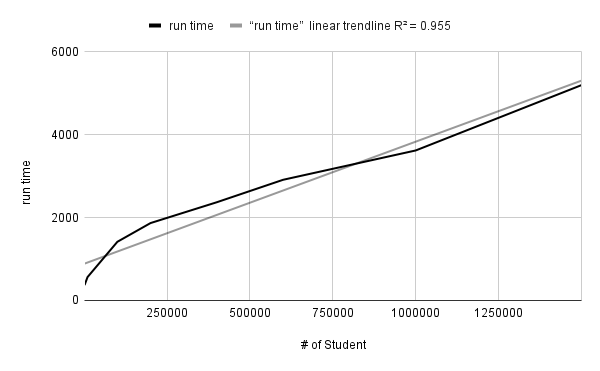
\includegraphics[width=10cm, height=6.4cm]{chart.png}}\\\

When we keep the number of rooms, classes, and time slots the same, and increase the number of students, we expect the running time would grow linearly as per time analysis suggests. The black line in the graph represents the actual run time of our program and the grey line represents a linear trend line. As the graph suggests, the time complexity is $O(s)$ when other constraints are fixed. The value $R^2 = 0.955$ suggests a very high fit for our analysis.
\\

\centerline{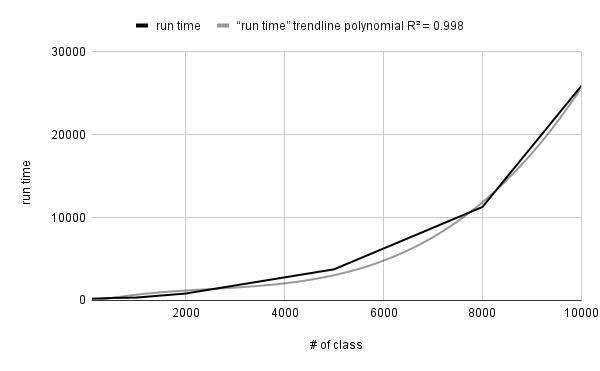
\includegraphics[width=10cm, height=6.4cm]{chart (2).png}}\\\

When we input fixed number of rooms, time slots and students, and increase the number of classes, we expect the running time to be $O(c^2logc^2)$. The black line in the graph represents the actual run time of our program and the grey line represents a cubic polynomial trend line. As the graph suggested, the time complexity of our program is very close to $c^3$ . $R^2 = 0.998$ suggests our high fit. But since we actually used ArrayList in the actual program, adding classes takes $O(c)$ rather than $O(1)$, which might affect the ultimate run time.

\subsection{Solution Quality Analysis}

\centerline{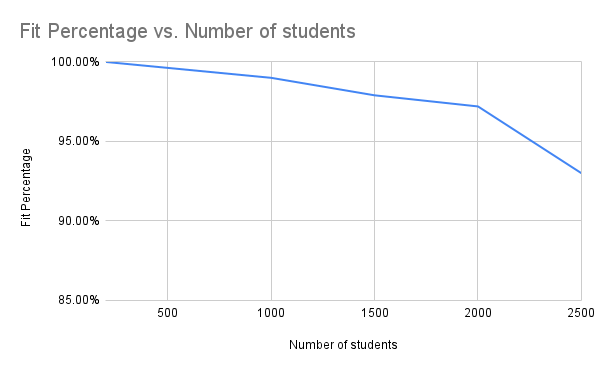
\includegraphics[width=10cm, height=6.4cm]{Fit Percentage vs. Number of students (1).png}}\\\

As illustrated in the graph above, with reasonable constraints, our program and algorithm can result in 98\% fit percentage on average. As the number of students increase, we reach a lower bound of 93\% of fit percentage.  \\

The reason why students can't take certain classes is mainly due to time conflict and not room capacity conflict because when we increase the room capacity in a reasonable range, the fit percentage didn't change much. 


\section{Real Life Scenarios}
When we extend our algorithm to run with the real Bryn Mawr/Haverford registration data in the past few years, there are several things need to be addressed in the code. 

\begin{enumerate}
    \item overlapping time: our previous assumption is that time slots are non-overlapping, but in reality the time is overlapped. We change the program so that if two classes' times is overlapped in any way, students can't take these two classes.
    \item identifiers: the real data has a string of numbers to identify a class, student, room, and professor. We added a step to store these identifiers as the name of the object and assigned another id starting from 0 for each object. 
    \item location constraints: since from the input list, we have locations followed by each course, we take those locations(rooms) as one of the constraints, i.e., classes could only take place in those locations. Thus, in the class \emph{Courses}, we added an arraylist to store the rooms available for each course to assign, and during scheduling, courses could only be assigned to those locations.
    \item number of classes in the preference list: In theoretical data, we assume each student must take 4 courses, but the real input data implies that the number of courses in each student's preference list varies. Some students take only 1 class and some take 5 classes. Thus, in order to calculate the fit percentage, we need to track how many classes students wish to take, rather than using $4\times s$.
\end{enumerate}

Based on the changes we made above, we try to extend the algorithm to accommodate other scenarios as potential suggestions we can give the registrar. 

\begin{enumerate}
    \item larger room capacity
    \item with/without location restriction
    \item splitting time slots
    \item adding labs without location restriction
    \item adding labs with location restriction
\end{enumerate}

Intuitively, increase the room capacity in a reasonable manner could increase the fit percentage because there are students unable to take a class because the room is not large enough. But our data suggests otherwise. When we track the number of time conflicts and the number of capacity conflicts, we noticed that when the student body is small (less than 30000), time conflicts surpass the capacity conflicts. Therefore, for a liberal art college with small student body, increasing the room capacity can't really make a large difference. 

We also hypothesized that if there is no location restriction, i.e. STEM classes has to be in Park Science Building, maybe we can have a more flexible schedule, thus resulting in a higher fit percentage. But as our data suggests, with or without the location restriction, we can achieve around 96\% fit percentage. So allowing flexibility in class location doesn't help.

Next we split the time slots so that, for example, a class can happen on Monday morning and Tuesday afternoon as long as the total lecture time for the class is 3 hours. We suspected that this way allows for more flexibility in class times; hence less classes would be scheduled at the conflict timeslots. However, we still get a 96\% fit percentage on average, which implies that a more flexible schedule does not make a difference.

Next, lab! We noticed some students has the same class in their preference list(actual registration list when using real data) twice, and we suspect that is the lab/discussion component of that class. There are two types of "labs". For CS labs and CHEM labs, for example, those subjects requires special equipment for labs thus they will need special rooms designed. For ECON labs and PSYC labs, since there is no specific lab requirement, labs can be assigned in any room available. We suspect that having labs for some courses may influence student's schedule, thus increasing schedule conflicts. On the other hand, we wonder whether if we assign all labs to certain lab rooms which will not be used as lecture rooms will influence the fit percentage. 

We have done two different approaches, one is lab with no location constraints, i.e., we assume that all labs are held in the same classroom as the lectures. The resulting fit percentage is around 96.5\%, which means that having labs with no location constraints  dose not influence the overall fit percentage. On the other hand, when we assign labs to special rooms, the result fit percentage is around 95.5\%, which, while still high, is lower than most of our results. We realized that having a lab with special lab rooms will slightly influence the overall fit percentage.

The reason why there is no significant change in fit percentage for the above implementation, we speculate is due to our original score is already high, and none of the changes can improve the score to a higher level. It is also possible because we use the data as all registered classes with registered locations, there might be some suitable available rooms to use while not in the data, which might help to improve our fit percentage.

Also, we assume courses could always fit in the less conflict timeslots. This could not be achieved if there are location constraints. According to the real data, the number of assigned classrooms for each course is limited, and thus should increase the number of schedule conflicts and decrease the overall fit.

We also speculate that since we did not create special lab timeslots but instead go under our modification with splitted timeslots, we wonder if we create special timeslots for labs as well as having combined timeslots will have some influence on the fit percentage. 

Further, we noticed that ESEM, the compulsory writing class for freshman, while having multiple sessions, doesn't reflect on the input data. Dealing with ESEM and college requirements might be something interesting and important for future research.


% \section{Future Plan and Thoughts}
% \begin{enumerate}
%     \item The given enrollment data has real life representations, e.g. names for professors, classes, and Weekday+start time and finish time of classes instead of random integer as IDs. We should implement a more realistic file reading method to translate the csv files.
    
%     \item lab/discussion time may not follow the time slot and will cause unexpected time conflicts.
    
%     Lab is a very special case to consider since lab rooms are not used for lectures and only used for labs. Discussion can use any classrooms if special equipment is not needed. The similarity of the two is that they don't take full class period and may different even the course shares the same time slot, the lab/discussion time period may not be the same.
%     In our present algorithm, we don't consider whether courses have or not have labs/discussions and for each course we only have 1 time slot assigned to each. We may will create special time slots for labs/discussions so that they can be assigned and this will be a special instance inside the object class we created for courses.
%     Another approach will be that we split the combined time slots and so that when we check schedule conflict, we will have to check all time slots. In that case, lab/discussion time slot will be added as a ordinary time slot.
%     Room will have less conflicts for lab since for example, CS labs are only for CS classes. Thus, we will add lab rooms as room objects with restriction only for special subjects and special courses. This is different for discussion since as mentioned, discussion can be held in any rooms.
    
%     \item there are some courses held only in one quarter (half of the semester)
    
    % Our intended approach will be to pair classes in first quarter and second quarter by least conflicts and consider them as a whole-semester course that will be scheduled together.
    
    % \item not every class can be scheduled in every room. (For example, English classes cannot be scheduled in Park). We can add a "subject" trait to each course and room. Rooms can have multiple subjects held in a array. Classes can only be assigned in rooms that have the matching "subject" in their array.
    
    % \item for one class taught by two professors
    
    % We may have two approaches. Pairing time slots for one professor but store it as single course. So that it is a single course with 2 different time slots assigned with different professors.
%     The other will be creating two objects of courses with same popularity. And they will be scheduled individually into the schedule.
    
%     \item time slots are not discrete, they may overlap 
%     We may use dynamic programming for scheduling with weight as popularity. 
    
%     \item Bryn Mawr College and Haverford College have equivalent classes
%     Even though some recommendation is made with a schedule time slot difference of 15 minutes, we could consider the schedule of blue bus to reduce the time overlap due to transportation. Personal experience indicates that we need more than 5 minutes to travel from Park Science Building to blue bus station. But the time difference between the end of the class and the blue bus schedule is 5 minutes. We found it really inconvenient if we want to have two consecutive courses in different campuses even with the 10 minutes difference between class and 15 minutes between schedule in different campuses. We don't have a very mature approach yet but we will discuss it later.
    
% \end{enumerate}

% \section{Things to further discuss}
% \begin{enumerate}
%     \item different courses may have different time length depends on the number of credits it offers.
%     \item lab/discussion time may not follow the time slot and will cause unexpected time conflicts - will assigning time slots specifically for labs help?
%     \item travel time for one building to another building or even campus - blue bus schedule?
%     \item different level of courses - students with the same major may favor similar electives and must-haves. For intro level courses, we might need to assign into less-likely conflicting slot in order to avoid conflicts
%     \item professor capability may cause one course is desired but unable to assign, even though this is not considered in the algorithm, but it is possible for some courses being unavailable.
%     \item special period - COVID - will course only have discussion/lab but remote lectures help to reduce the conflict of the schedule?
%     \item will open and closed time for dining hall influence student's schedule?
%     \item for each room, the available time slot may be different. This will happen since course assigned to the room may not share the same duration time.
%     \item the above algorithm restricts the class size by the capacity of the room. Yet in real life, the class size depends on the mode of the course, for example, and not every popular class can be assigned into large rooms, since different subjects have different rooms. 
% \end{enumerate}

% \section{Topics}
% \begin{enumerate}
%     \item fix time slot to 1.5 hours each. Instead of each class being assigned to a single time slot, our modification will assign each class to two 1.5 hour time slots on different days
    % \item If a class has a lab or discussion session, then the class will be schedule with an additional time slot (for a total of 3 times slot)
    
    % Lab is a very special case to consider since lab rooms are not used for lectures and only used for labs. Discussion can use any classrooms if special equipment is not needed. The similarity of the two is that they don't take full class period and may different even the course shares the same time slot, the lab/discussion time period may not be the same.
    % In our present algorithm, we don't consider whether courses have or not have labs/discussions and for each course we only have two 1.5 hour time slots assigned to each. 
    % In our modification, we will implement an additional boolean characteristic of each class called $hasLab$. If a class has a lab, then it will be assigned an additional time slot, and students will simultaneously be enrolled in this time slot when they are enrolled in the class. Conflicts with the new time slot will be counted into the number of conflicts for the whole class.
    % Room will have less conflicts for lab since for example, CS labs are only for CS classes. Thus, we will add lab rooms as room objects with restriction only for special subjects and special courses. This is different for discussion since as mentioned, discussion can be held in any rooms.
    % \item labs location constraints - we apply two labs for each subject for them to use -> then we increment to 4
    % \item Add 2 extra seats to certain classes
    % \item Location constraints. Some classes cannot be assigned to certain rooms. For example, English classes cannot be assigned to any room in Park. We will implement an additional array characteristic of each class called $validLocations$. When matching classes to rooms, we first check if the room is in a building in the list of $validLocations$ of the class.
% \end{enumerate}
\end{document}
